\documentclass[12pt,a4paper]{report}
\usepackage{fontspec}
\IfFontExistsTF{TeX Gyre Termes}{\setmainfont{TeX Gyre Termes}}{\setmainfont{Liberation Serif}}
\IfFontExistsTF{TeX Gyre Heros}{\setsansfont{TeX Gyre Heros}}{\setsansfont{Liberation Sans}}
\setmonofont[Scale=0.84]{DejaVu Sans Mono}
\usepackage[vietnamese]{babel}
\usepackage[a4paper,margin=1in]{geometry}
\usepackage{amsmath,amssymb,mathtools,bm}
\usepackage{booktabs,tabularx,array,longtable}
\usepackage{graphicx,float}
\usepackage[hidelinks]{hyperref}
\usepackage{fancyhdr,setspace,titlesec,caption,microtype,needspace}
\usepackage{enumitem}
\setstretch{1.15}
\setlength{\parskip}{0.3em}
\setlength{\parindent}{0pt}
\setlength{\headheight}{16pt}
\setcounter{tocdepth}{1}
\setcounter{secnumdepth}{2}
\captionsetup{font=small,labelfont=bf}
\numberwithin{equation}{chapter}
\titleformat{\chapter}[display]{\normalfont\bfseries}{\filleft\Large Chương \thechapter}{0.3em}{\filright\huge}[\vspace{0.4em}\titlerule]
\titlespacing*{\chapter}{0pt}{-10pt}{20pt}
\titleformat{\section}{\large\bfseries}{\thesection}{0.6em}{}
\titleformat{\subsection}{\normalsize\bfseries}{\thesubsection}{0.6em}{}
\pagestyle{fancy}
\fancyhf{}
\lhead{\small CO5177 · Text}
\rhead{\small Học kỳ 261 · Text}
\cfoot{\thepage}
\fancypagestyle{plain}{\fancyhf{}\lhead{\small CO5177 · Text}\rhead{\small Học kỳ 261 · Text}\cfoot{\thepage}}
\newcommand{\R}{\mathbb{R}}
\newcommand{\norm}[1]{\left\lVert #1 \right\rVert}
\newcommand{\code}[1]{\texttt{\detokenize{#1}}}
\newcommand{\resultfigure}[3]{\begin{figure}[htbp]\centering\includegraphics[width=#3\textwidth]{generated/figures/#1.png}\caption{#2}\end{figure}}
\hypersetup{pdftitle={CO5177 - Bao cao Text},pdfauthor={Huynh Thanh Dat; Luong Minh Duy}}
\emergencystretch=2em

\begin{document}
\hypersetup{pageanchor=false}
\begin{titlepage}\centering
{\large ĐẠI HỌC QUỐC GIA THÀNH PHỐ HỒ CHÍ MINH\par}
{\large\bfseries TRƯỜNG ĐẠI HỌC BÁCH KHOA\par}
{\large KHOA KHOA HỌC VÀ KỸ THUẬT MÁY TÍNH\par}
\vspace{1cm}
\includegraphics[width=3cm]{assets/hcmut-logo.png}\par
\vspace{.8cm}{\large\bfseries NỀN TẢNG LẬP TRÌNH CHO PHÂN TÍCH\par}
{\large\bfseries VÀ TRỰC QUAN DỮ LIỆU\par}{\large Mã môn học: CO5177\par}
\vspace{1cm}\rule{\textwidth}{.6pt}\par\vspace{.4cm}
{\Huge\bfseries BÁO CÁO TEXT\par}\vspace{.5cm}
{\Large Phân loại tin tức VietnamNet bằng PhoBERT\\[.3em] Fine-tuning, temperature scaling và ngưỡng theo lớp\par}\vspace{.4cm}\rule{\textwidth}{.6pt}\par
\vspace{.8cm}{\large Học kỳ 261 · Năm học 2026–2027\par}\vspace{.7cm}
\begin{tabular}{ll}Giảng viên: & Lê Thành Sách\\[.5em]
Thành viên: & Huỳnh Thành Đạt · 2570161\\ & Lương Minh Duy · 2570083\end{tabular}
\vfill{\small Thành phố Hồ Chí Minh, tháng 10 năm 2026\par}
\end{titlepage}\hypersetup{pageanchor=true}
\pagenumbering{roman}{\footnotesize\setstretch{1}\tableofcontents}\clearpage\pagenumbering{arabic}

\chapter{Bài toán và quy trình thực nghiệm}
\section{Mục tiêu}
Bài toán phân loại 212.705 bài báo VietnamNet vào 19 chuyên mục. PhoBERT Base v2 và đầu phân loại được fine-tune trên tiêu đề cùng nội dung đầu--cuối; temperature scaling và ngưỡng theo lớp được dùng để hiệu chỉnh xác suất và quyết định.

Lần chạy Kaggle với hai Tesla T4 diễn ra từ 26 đến 27/4/2026 theo giờ Việt Nam. Báo cáo sử dụng lại notebook, log và hình của lần chạy đó. Bộ đối chứng mới trên 7.600 tiêu đề được trình bày riêng ở phụ lục do khác đầu vào và cách chia tập.

\section{Các bước trong notebook}
\begin{table}[htbp]\centering\footnotesize
\begin{tabularx}{\textwidth}{clX}\toprule
Section & Nội dung & Kết quả trung gian\\\midrule
0 & Thiết lập & Thư viện, thiết bị, đường dẫn, tham số và kiểm tra parquet.\\
1 & Nạp dữ liệu & 19 tệp chuyên mục, số bài và số trường thiếu.\\
2 & Khảo sát dữ liệu & Phân bố lớp, độ dài và thống kê theo chuyên mục.\\
3 & Tiền xử lý & Chuẩn hóa, PyVi, cache văn bản đã tách từ.\\
4 & Dataset & Chia 85/15, Head--Tail, class weight và tensor cache.\\
5 & Fine-tune & WeightedTrainer, checkpoint, log bảy epoch.\\
6 & Đánh giá & Accuracy, F1, confusion, đường cong và lỗi theo lớp.\\
7 & Xuất mô hình & Model, tokenizer, nhãn và smoke test.\\
8 & Calibration & Temperature, ECE, ngưỡng theo lớp và chỉ số sau hiệu chỉnh.\\
9 & Chẩn đoán & Lớp khó, đánh đổi precision/recall và cặp nhầm lẫn.\\\bottomrule
\end{tabularx}
\caption{Trình tự xử lý của notebook gồm 36 cell, trong đó 25 cell code có output đã lưu.}
\end{table}

\section{Thiết lập môi trường -- Section 0}
Notebook kiểm tra thư viện trước khi xử lý dữ liệu; các gói còn thiếu như Transformers, Accelerate và PyVi được cài ở cell đầu. Thiết bị được phát hiện theo CUDA, MPS hoặc CPU. Lần chạy ghi nhận Python 3.12.12, PyTorch 2.10.0+cu128, hai Tesla T4, khoảng 14,6 GiB VRAM mỗi GPU. Cấu hình thực chạy dùng FP16; BF16 bị tắt vì T4 thuộc kiến trúc Turing.

Section 0.3 tập trung đường dẫn, cache và các biến cấu hình. Dataset được tải từ Hugging Face khi chưa có parquet cục bộ; lần đo để số dòng tối đa mỗi lớp bằng 0, tức không giới hạn theo lớp.

\chapter{Dữ liệu và khảo sát ban đầu}
\section{Nguồn dữ liệu -- Section 1}
Corpus VietnamNet do Huỳnh Thành Đạt thu thập gồm tiêu đề, nội dung, URL và chuyên mục \cite{vietnamnet}. Notebook đọc 19 tệp parquet theo batch 20.480 dòng để giảm mức sử dụng RAM. Nhãn được ánh xạ từ tên tệp sang tên chuyên mục tiếng Việt; tên chuyên mục và URL không được nối vào văn bản đầu vào.

Log nạp dữ liệu ghi 212.705 bài, 1.167 tiêu đề thiếu và 7 nội dung thiếu. Không có bài thiếu cả tiêu đề lẫn nội dung nên không có dòng bị loại ở bước này. Sau tách từ vẫn còn 212.705 bài hợp lệ. Trường hợp thiếu tiêu đề được giữ nếu nội dung còn sử dụng được; cách xử lý này khác với bài đối chứng chỉ dùng tiêu đề.

Notebook tải dataset theo tên repository nhưng không ghi revision hoặc SHA256 các parquet của lần chạy cũ. Số dòng theo từng tệp khớp với bản corpus dùng trong kiểm tra hiện tại; điều đó chưa chứng minh hai bản có nội dung byte-identical. Dataset card không nêu rõ license phân phối lại nội dung báo chí, nên raw corpus được giữ ngoài Git.

\section{Phân bố chuyên mục -- Section 2.1}
Các lớp lớn có khoảng 12.500 bài, trong khi Dân tộc -- Tôn giáo có 3.355 bài và Bảo vệ người tiêu dùng có 3.873 bài. Tỷ lệ lớp lớn nhất so với nhỏ nhất xấp xỉ 3,73 lần. Vì vậy, báo cáo dùng cả macro-F1 và weighted-F1; accuracy hoặc weighted-F1 riêng lẻ có thể che khuất kết quả của các lớp ít mẫu.
\begin{figure}[htbp]\centering
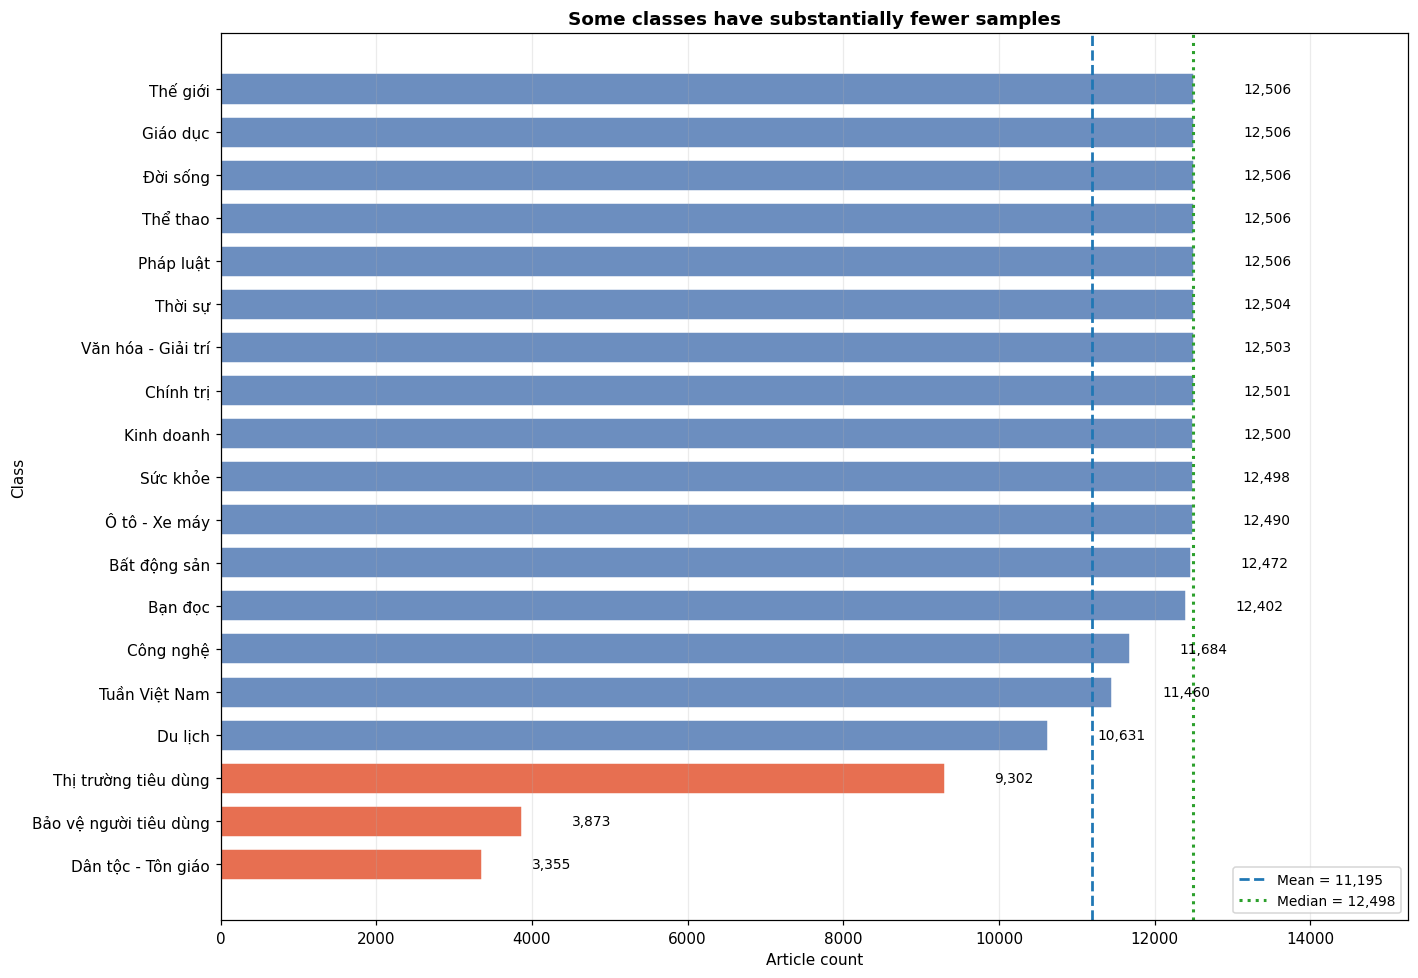
\includegraphics[width=.96\textwidth]{reused/figures/01_class_distribution.png}
\caption{Phân bố 19 chuyên mục, trích nguyên hình đã lưu trong notebook.}\end{figure}
\begin{table}[htbp]\centering\small
\begin{tabularx}{\textwidth}{Xrr}\toprule
Chuyên mục & Số bài & Tỷ lệ\\\midrule
Bạn đọc & 12,402 & 5.83\%\\
Bảo vệ người tiêu dùng & 3,873 & 1.82\%\\
Bất động sản & 12,472 & 5.86\%\\
Chính trị & 12,501 & 5.88\%\\
Công nghệ & 11,684 & 5.49\%\\
Du lịch & 10,631 & 5.00\%\\
Dân tộc - Tôn giáo & 3,355 & 1.58\%\\
Giáo dục & 12,506 & 5.88\%\\
Kinh doanh & 12,500 & 5.88\%\\
Pháp luật & 12,506 & 5.88\%\\
Sức khỏe & 12,498 & 5.88\%\\
Thế giới & 12,506 & 5.88\%\\
Thể thao & 12,506 & 5.88\%\\
Thị trường tiêu dùng & 9,302 & 4.37\%\\
Thời sự & 12,504 & 5.88\%\\
Tuần Việt Nam & 11,460 & 5.39\%\\
Văn hóa - Giải trí & 12,503 & 5.88\%\\
Ô tô - Xe máy & 12,490 & 5.87\%\\
Đời sống & 12,506 & 5.88\%\\
\bottomrule\end{tabularx}

\caption{Số bài theo chuyên mục đọc từ log nạp parquet của lần chạy.}\end{table}

\section{Độ dài văn bản -- Section 2.2}
Thống kê độ dài được tính trên văn bản nguồn trước khi rút gọn nội dung: trung vị 625 từ, phân vị 90 là 1.218 từ và phân vị 95 là 1.505 từ. Khoảng 89,9\% bài dài hơn 256 từ. Đơn vị này là từ tách theo khoảng trắng, không đồng nhất với subword token của PhoBERT.

Để giảm RAM, phần body giữ tối đa 220 từ đầu và 80 từ cuối trước khi tiền xử lý. Sau khi nối tiêu đề, làm sạch và tách từ, notebook kiểm tra 1.000 văn bản bằng tokenizer PhoBERT: trung bình 246,3 token, trung vị 254, khoảng 46,3\% vượt 256 token. Hai tỷ lệ 89,9\% và 46,3\% mô tả hai giai đoạn và hai đơn vị khác nhau.
Hình histogram gốc được giữ tại phụ lục hình để đối chiếu.


\chapter{Tiền xử lý và biểu diễn đầu vào}
\section{Làm sạch, tách từ và cache -- Section 3}
Tiêu đề được nối một lần với phần body đầu--cuối. Hàm xử lý chuyển chữ thường, thay dấu câu bằng khoảng trắng, loại chữ số, chạy \code{pyvi.ViTokenizer} và gộp khoảng trắng. Stopword được giữ để bảo toàn ngữ cảnh cho PhoBERT \cite{phobert,pyvi}. Việc loại chữ số có thể làm mất năm, giá trị tiền hoặc tỷ số; chưa có ablation để định lượng ảnh hưởng riêng của lựa chọn này.

Tiền xử lý chạy theo batch 512 bài với hai worker. Kết quả gồm văn bản đã tách từ, nhãn và ánh xạ label--ID được lưu vào cache. Metadata cache chứa giới hạn mẫu theo lớp và số từ đầu/cuối. Các cache của notebook cũ không gắn SHA256 toàn bộ nội dung nguồn, vì vậy khi thay dataset cần xóa cache và tạo lại, thay vì suy ra tính hợp lệ chỉ từ các tham số.

\section{Chia tập -- Section 4}
\code{train_test_split} chia phân tầng theo chuyên mục, seed 42, tỷ lệ 85/15. Hai tập có 180.799 bài train và 31.906 bài mang tên test. Thứ tự lớp được sắp xếp rồi ánh xạ về ID 0--18; cùng thứ tự được dùng cho loss, logits, confusion và ngưỡng.

Trong notebook, tập 31.906 bài còn được truyền vào \code{eval_dataset} để chọn checkpoint, early stopping, temperature scaling và tìm ngưỡng. Do đó, báo cáo gọi đây là \emph{tập đánh giá}, giữ tên test khi mô tả mã nguồn; nó không phải một tập test độc lập chưa tham gia lựa chọn mô hình. Notebook không thực hiện loại trùng URL/văn bản trước split và không lưu ID từng split. Mức giao nhau giữa các nhóm trùng của lần chạy cũ chưa được kiểm chứng.

\section{Head--Tail và tensor dataset}
Sau tách từ, tokenizer chuyển văn bản thành subword ID. Nếu có tối đa 254 token nội dung, chuỗi được thêm token đặc biệt và pad đến độ dài 256. Với chuỗi dài hơn, dataset giữ 127 token đầu và 127 token cuối:
\[
x=[\mathrm{CLS}]\;\Vert\;t_{1:127}\;\Vert\;t_{L-126:L}\;\Vert\;[\mathrm{SEP}].
\]
Attention mask bằng 1 tại token thật và 0 tại padding. \code{HeadTailDataset} lưu input IDs, attention mask và nhãn thành tensor; cache train/test giúp tránh token hóa lại. Có hai mức rút gọn: 220+80 \emph{từ} ở loader và 127+127 \emph{subword token} ở dataset. Mô hình không đọc toàn bộ body dài sau hai bước này.

\chapter{Fine-tune và đánh giá mô hình}
\section{Cân bằng lớp}
Class weight được tính trên nhãn train theo \code{compute_class_weight(balanced)}, sau đó nhân hệ số bổ sung:
\[
w_c=\frac{N_{\mathrm{train}}}{K\,n_c}\,b_c,\qquad K=19.
\]
Hệ số $b_c$ bằng 1,35 cho Dân tộc -- Tôn giáo; 1,15 cho Kinh doanh và Thời sự; 1,10 cho Thị trường tiêu dùng và Đời sống; các lớp khác bằng 1. Đây là các tham số cố định trong notebook, chưa có đối chứng tách riêng lợi ích của manual boost.

\section{Kiến trúc và loss -- Section 5}
\code{AutoModelForSequenceClassification} khởi tạo PhoBERT Base v2 với 19 nhãn. Đầu phân loại RoBERTa nhận biểu diễn token đầu, qua dropout, dense, tanh và lớp chiếu 19 logits. Encoder và đầu phân loại cùng được cập nhật khi fine-tune; không có Logistic Regression ở cuối pipeline này. Logistic Regression chỉ thuộc thực nghiệm đối chứng dùng encoder đóng băng ở phụ lục.

\code{WeightedTrainer.compute_loss} lấy logits và tính cross-entropy có trọng số. Với batch $B$ và cách giảm trung bình theo trọng số của PyTorch, loss là
\[
\mathcal{L}_B=-\frac{\sum_{i\in B}w_{y_i}\log p_\theta(y_i\mid x_i)}{\sum_{i\in B}w_{y_i}}.
\]
Việc chuyển class weight sang cùng thiết bị với logits được thực hiện trong hàm loss.

\begin{table}[htbp]\centering\small
\begin{tabularx}{\textwidth}{Xl}\toprule
Tham số & Giá trị thực chạy\\\midrule
Mô hình & PhoBERT Base v2, khoảng 135 triệu tham số\\
Số epoch / optimizer steps & 7 / 19.775\\
Độ dài input & 256 token\\
Batch mỗi GPU / tích lũy gradient & 16 / 2\\
GPU / batch hiệu dụng toàn cục & 2 Tesla T4 / $16\times2\times2=64$\\
Batch đánh giá mỗi GPU & 32\\
Learning rate / weight decay & $2\times10^{-5}$ / 0,01\\
Warmup / optimizer & 200 bước / fused AdamW\\
Precision & FP16; không dùng BF16\\
Checkpoint và đánh giá & Mỗi epoch; chọn macro-F1 lớn nhất\\
Early stopping / số checkpoint giữ & Patience 3 / 1\\
DataLoader workers & 0\\
Gradient checkpointing / torch compile & Tắt / tắt\\\bottomrule
\end{tabularx}
\caption{Thông số lấy từ cấu hình và log CUDA của notebook đã chạy.}\end{table}

\section{Đường cong và chọn checkpoint}
Trainer đánh giá sau mỗi epoch, giữ checkpoint có macro-F1 cao nhất và nạp lại trước khi xuất model. Log ghi đủ bảy epoch, tổng thời gian fine-tune khoảng 38.115 giây, tương đương 635,2 phút. Toàn bộ notebook mất khoảng 11 giờ 1 phút, bao gồm tải dữ liệu, tiền xử lý, suy luận và calibration. Các số này thuộc lần chạy Kaggle, không phải thời gian chạy trên máy cục bộ hoặc Vast.

\begin{table}[htbp]\centering\small
\begin{tabularx}{\textwidth}{Xrrrr}\toprule
Epoch & Train loss* & Eval loss & Accuracy & Macro-F1\\\midrule
1 & 0.833146 & 0.404629 & 0.880493 & 0.868397\\
2 & 0.643082 & 0.354720 & 0.894346 & 0.885470\\
3 & 0.458360 & 0.338845 & 0.900332 & 0.891702\\
4 & 0.335830 & 0.363673 & 0.904344 & 0.897606\\
5 & 0.263415 & 0.371614 & 0.904751 & 0.897426\\
6 & 0.205018 & 0.413617 & 0.904407 & 0.897382\\
7 & 0.191186 & 0.432415 & 0.905190 & 0.898581\\
\bottomrule\end{tabularx}

\caption{Bảng Trainer in sau từng epoch, giữ sáu chữ số thập phân. *Train loss là thống kê được Trainer in ở thời điểm đó; không coi là trung bình toàn bộ epoch.}\end{table}
\begin{figure}[htbp]\centering
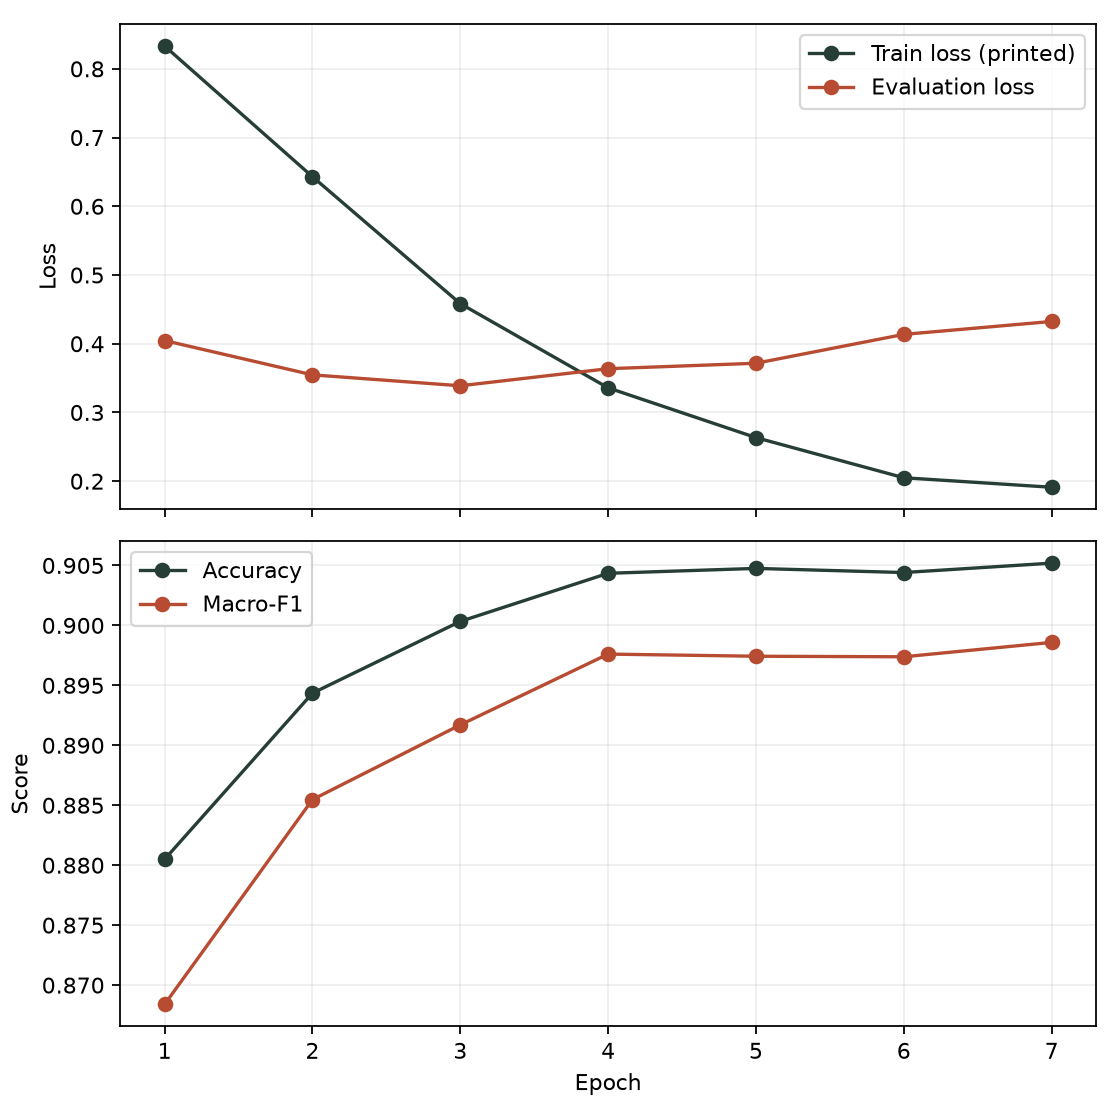
\includegraphics[width=.9\textwidth]{reused/tables/epoch_curves.png}
\caption{Vẽ lại từ bảng epoch đã lưu, dùng cùng trục epoch cho các đường. Đây là cùng số liệu, không phải lần huấn luyện bổ sung.}\end{figure}

Macro-F1 tăng từ 0,868397 ở epoch 1 lên 0,898581 ở epoch 7; epoch 7 đạt giá trị cao nhất trong bảy mốc. Eval loss nhỏ nhất tại epoch 3 (0,338845) rồi tăng tới 0,432415, trong khi train loss tiếp tục giảm. Diễn biến này cho thấy chất lượng xác suất và chỉ số dự đoán nhãn không cải thiện đồng thời; tăng độ tự tin ở các dự đoán sai có thể làm NLL tăng dù accuracy vẫn nhích lên. Cần thêm validation độc lập để đánh giá độ ổn định của lựa chọn checkpoint.

\section{Kết quả trước hiệu chỉnh -- Section 6}
Suy luận trên 31.906 bài dùng argmax của logits, đạt accuracy 90,52\%, weighted-F1 0,905308 và macro-F1 0,898581. Macro-F1 thấp hơn weighted-F1 cho thấy các lớp ít mẫu hoặc khó phân biệt vẫn kéo giảm kết quả trung bình theo lớp.
\begin{figure}[htbp]\centering
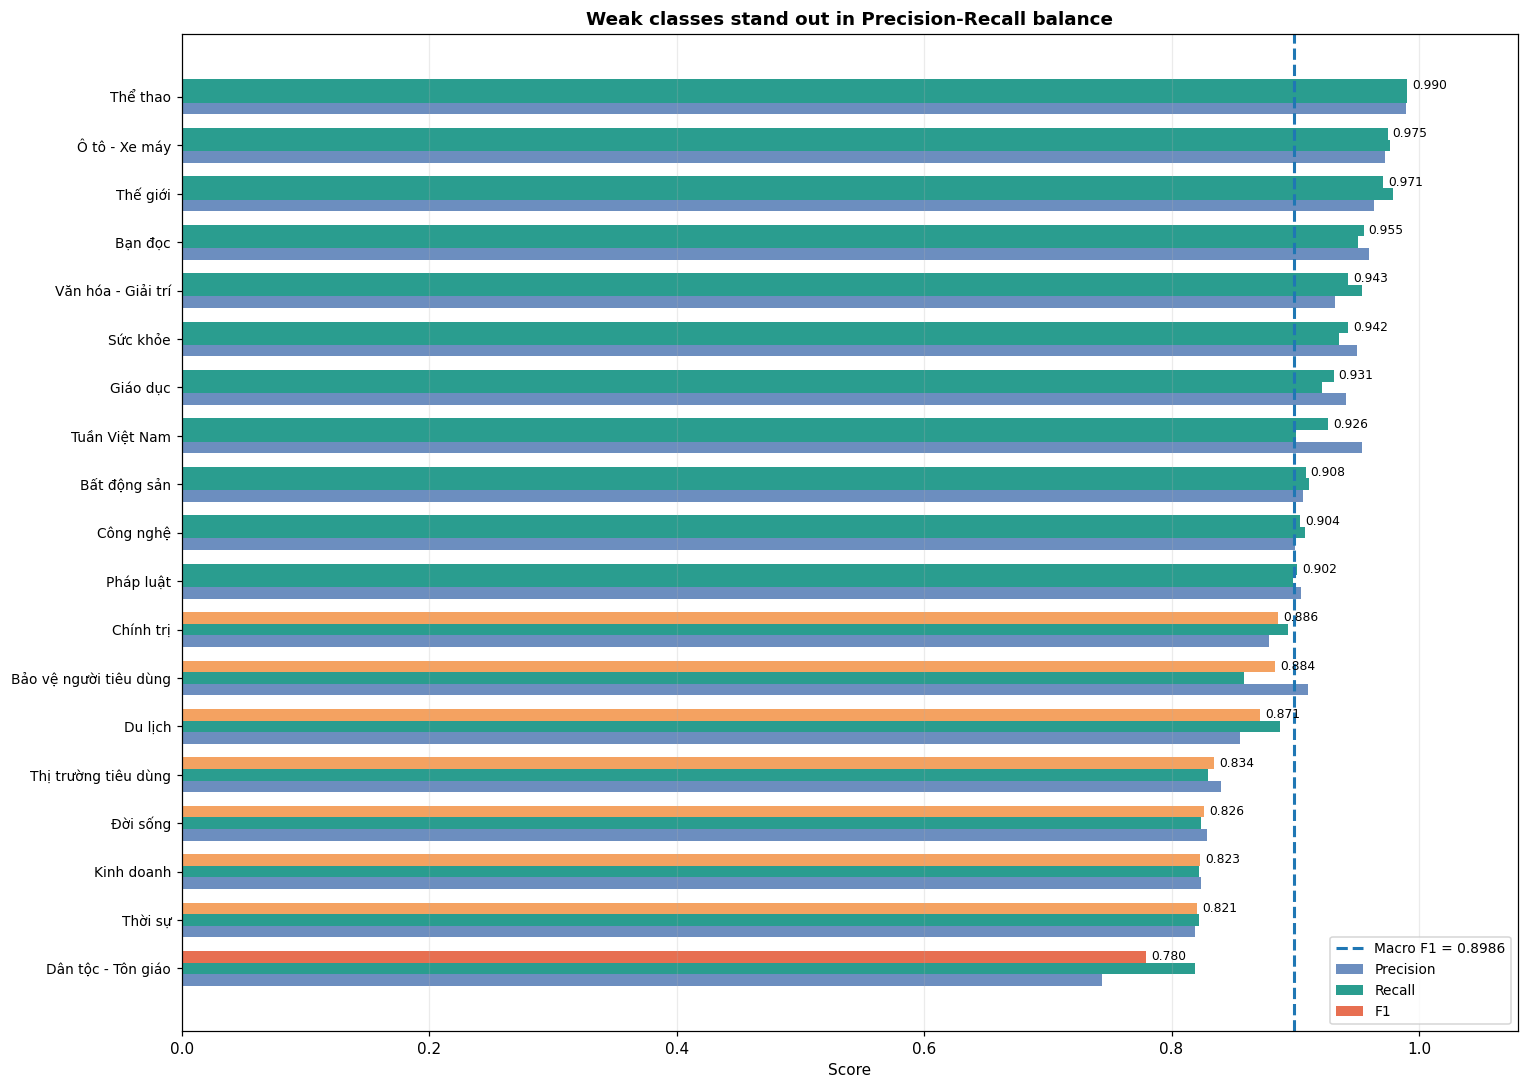
\includegraphics[width=.95\textwidth]{reused/figures/04_f1_per_class.png}
\caption{Precision, recall và F1 theo lớp trước hiệu chỉnh, từ notebook gốc.}\end{figure}
\begin{figure}[htbp]\centering
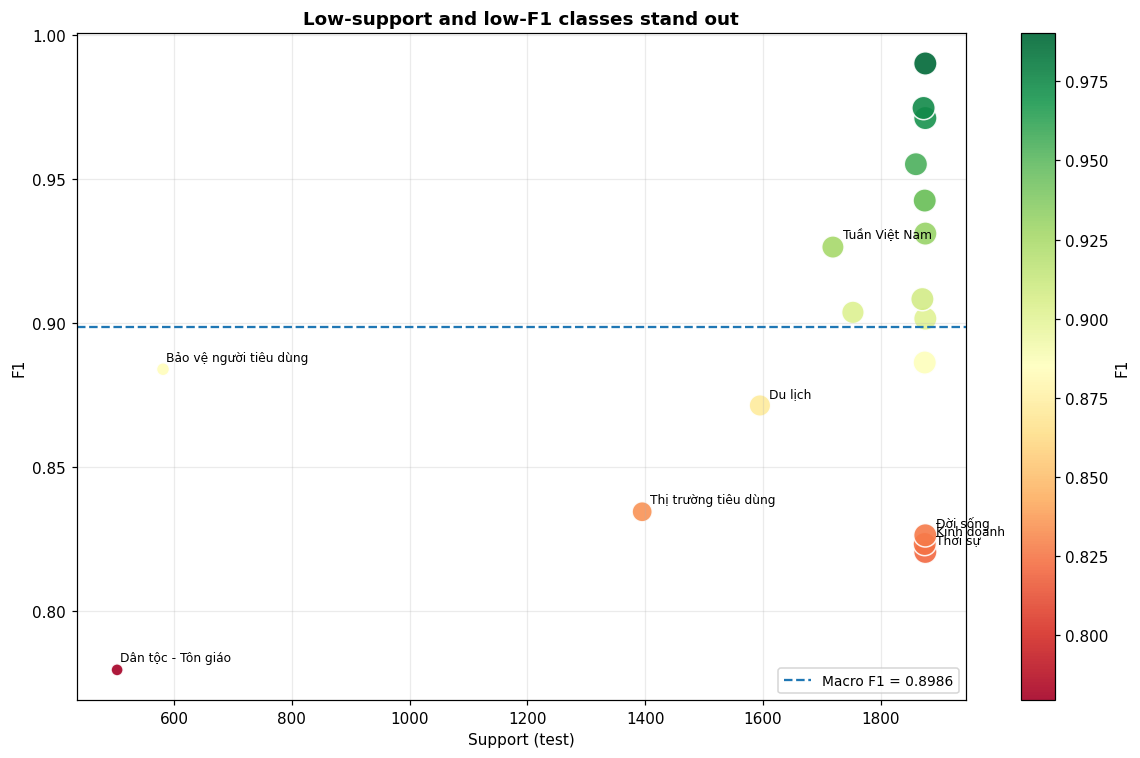
\includegraphics[width=.85\textwidth]{reused/figures/07_support_vs_f1.png}
\caption{Số mẫu đánh giá và F1 trước hiệu chỉnh. Kích thước lớp không giải thích toàn bộ khác biệt giữa các chuyên mục.}\end{figure}

Thể thao đạt F1 0,9901, trong khi Dân tộc -- Tôn giáo chỉ đạt 0,7796 với 503 mẫu đánh giá. Kinh doanh, Thời sự, Đời sống và Thị trường tiêu dùng có F1 khoảng 0,82--0,83. Những chuyên mục này có phạm vi nội dung giao nhau; confusion cho biết cặp cần xem lại, chưa đủ để kết luận nhãn nguồn sai.

\section{Xuất mô hình -- Section 7}
Notebook lưu trọng số dạng safetensors, config kiến trúc, tokenizer, ánh xạ nhãn, chiến lược Head--Tail và metadata tiền xử lý. Ba bài lấy mẫu từ dữ liệu nguồn được dùng để kiểm tra nhanh đường suy luận; đây là smoke test, không phải một phép đo accuracy độc lập. Sau Section 8, package được bổ sung temperature, ngưỡng, classification report và confusion dạng JSON.

Model package trong repository ứng dụng có trọng số khoảng 540 MB. Khi chuyển bài, metadata được giữ nguyên và checkpoint được xác định bằng SHA256 trong manifest; trọng số, raw corpus và tensor cache nằm ngoài Git của CO5177. Source của toàn bộ 36 cell trong file đã chạy khớp notebook tại commit \code{e171688} của repository ứng dụng \cite{application}.

\chapter{Hiệu chỉnh xác suất và ngưỡng quyết định}
\section{Temperature scaling -- Section 8.0}
Cho vector logits $z_i$, xác suất sau hiệu chỉnh được tính bởi
\[
p_{i,c}(T)=\frac{\exp(z_{i,c}/T)}{\sum_{k=1}^{K}\exp(z_{i,k}/T)},\qquad T>0.
\]
Notebook tìm một scalar $T$ bằng \code{scipy.optimize.minimize_scalar}, phương pháp bounded trên khoảng $[0{,}5;5{,}0]$, nhằm giảm negative log-likelihood:
\[
T^*=\arg\min_T-\frac{1}{N}\sum_{i=1}^{N}\log p_{i,y_i}(T).
\]
Kết quả $T^*=1{,}4583027$ làm phân bố xác suất mềm hơn. Temperature dương dùng chung cho mọi lớp không thay đổi thứ tự logits, nên argmax và accuracy không thay đổi chỉ nhờ bước này.

Notebook đo ECE bằng 15 bin độ tin cậy, dựa trên xác suất lớn nhất và tỷ lệ đúng trong mỗi bin:
\[
\mathrm{ECE}=\sum_{b=1}^{15}\frac{|B_b|}{N}\left|\operatorname{acc}(B_b)-\operatorname{conf}(B_b)\right|.
\]
NLL giảm từ 0,3828 xuống 0,3237; ECE giảm từ 0,0608 xuống 0,0218 trên tập dùng để tìm $T$. Các giá trị này được in bốn chữ số thập phân trong notebook. Mức giảm phản ánh độ khớp trên chính tập calibration, chưa phải bằng chứng về độ tin cậy trên dữ liệu chưa thấy.

\section{Ngưỡng riêng cho từng lớp -- Section 8.1}
Sau temperature scaling, quyết định cuối dùng
\[
\widehat{y}_i=\arg\max_c\frac{p_{i,c}(T^*)}{\tau_c}.
\]
Ngưỡng lớn hơn 1 làm lớp khó được chọn hơn; nhỏ hơn 1 làm lớp dễ được chọn hơn so với các lớp khác. Tỷ số $p/\tau$ là điểm dùng để xếp hạng, không phải xác suất đã chuẩn hóa. Quy tắc luôn chọn đúng một lớp, không biến bài toán thành multi-label.

Các ngưỡng khởi tạo bằng 1. Notebook chạy ba lượt qua 19 lớp; với mỗi lớp, thử 200 ứng viên cách đều từ 0,3 đến 3,5, giữ các ngưỡng lớp khác cố định và chọn ứng viên tăng F1 của lớp đang xét hơn $10^{-5}$. Đây là tìm kiếm tuần tự theo tọa độ, tối ưu F1 từng lớp tại thời điểm xét; không bảo đảm tối ưu toàn cục macro-F1. Thay ngưỡng một lớp có thể thay đổi precision/recall của các lớp còn lại.

\section{Kết quả trước và sau -- Section 8.2}
\begin{table}[htbp]\centering\small
\begin{tabularx}{\textwidth}{Xrrr}\toprule
Chỉ số & Trước hiệu chỉnh & Sau hiệu chỉnh & Chênh lệch\\\midrule
Accuracy & 0.905190 & 0.908638 & +0.003448\\
Weighted-F1 & 0.905308 & 0.908457 & +0.003149\\
Macro-F1 & 0.898581 & 0.901626 & +0.003046\\
\bottomrule\end{tabularx}

\caption{Chỉ số trên cùng tập đánh giá trước và sau temperature kết hợp ngưỡng theo lớp.}\end{table}
Accuracy tăng từ 90,5190\% lên 90,8638\%, tương đương 0,3448 điểm phần trăm. Macro-F1 tăng từ 0,898581 lên 0,901626. Vì temperature đơn lẻ giữ nguyên argmax, thay đổi chỉ số phân loại đến từ bước điều chỉnh ngưỡng.

\begin{table}[htbp]\centering\small\setlength{\tabcolsep}{4pt}
\begin{tabularx}{\textwidth}{Xrrrr}\toprule
Chuyên mục & Số mẫu & F1 trước & F1 sau & Ngưỡng\\\midrule
Bạn đọc & 1860 & 0.9552 & 0.9596 & 3.3070\\
Bảo vệ người tiêu dùng & 581 & 0.8840 & 0.8857 & 1.5543\\
Bất động sản & 1871 & 0.9083 & 0.9093 & 0.8307\\
Chính trị & 1875 & 0.8863 & 0.8904 & 1.7472\\
Công nghệ & 1753 & 0.9037 & 0.9070 & 0.5894\\
Du lịch & 1595 & 0.8714 & 0.8725 & 1.2648\\
Dân tộc - Tôn giáo & 503 & 0.7796 & 0.7813 & 1.1362\\
Giáo dục & 1876 & 0.9311 & 0.9344 & 1.0879\\
Kinh doanh & 1875 & 0.8233 & 0.8286 & 0.6698\\
Pháp luật & 1876 & 0.9016 & 0.9093 & 0.3965\\
Sức khỏe & 1875 & 0.9425 & 0.9445 & 1.5704\\
Thế giới & 1876 & 0.9712 & 0.9729 & 2.1814\\
Thể thao & 1876 & 0.9901 & 0.9912 & 3.2427\\
Thị trường tiêu dùng & 1395 & 0.8345 & 0.8378 & 2.2136\\
Thời sự & 1876 & 0.8205 & 0.8235 & 1.5060\\
Tuần Việt Nam & 1719 & 0.9264 & 0.9327 & 0.7342\\
Văn hóa - Giải trí & 1875 & 0.9425 & 0.9438 & 0.9111\\
Ô tô - Xe máy & 1873 & 0.9747 & 0.9765 & 2.4709\\
Đời sống & 1876 & 0.8263 & 0.8300 & 2.7764\\
\bottomrule\end{tabularx}

\caption{F1 và ngưỡng của 19 lớp. F1 trước được khôi phục từ bảng in bốn chữ số; F1 sau và ngưỡng lấy từ JSON xuất cùng model.}\end{table}
Pháp luật tăng F1 từ khoảng 0,9016 lên 0,9093, với ngưỡng 0,3965. Recall tăng từ khoảng 0,8982 lên 0,9622 nhưng precision giảm từ khoảng 0,9049 xuống 0,8620. Thời sự có ngưỡng 1,5060; precision tăng nhưng recall giảm xuống 0,7772. Hai ví dụ cho thấy hiệu chỉnh quyết định dịch chuyển lỗi giữa các lớp, không chỉ đồng loạt cải thiện khả năng biểu diễn.

\begin{figure}[htbp]\centering
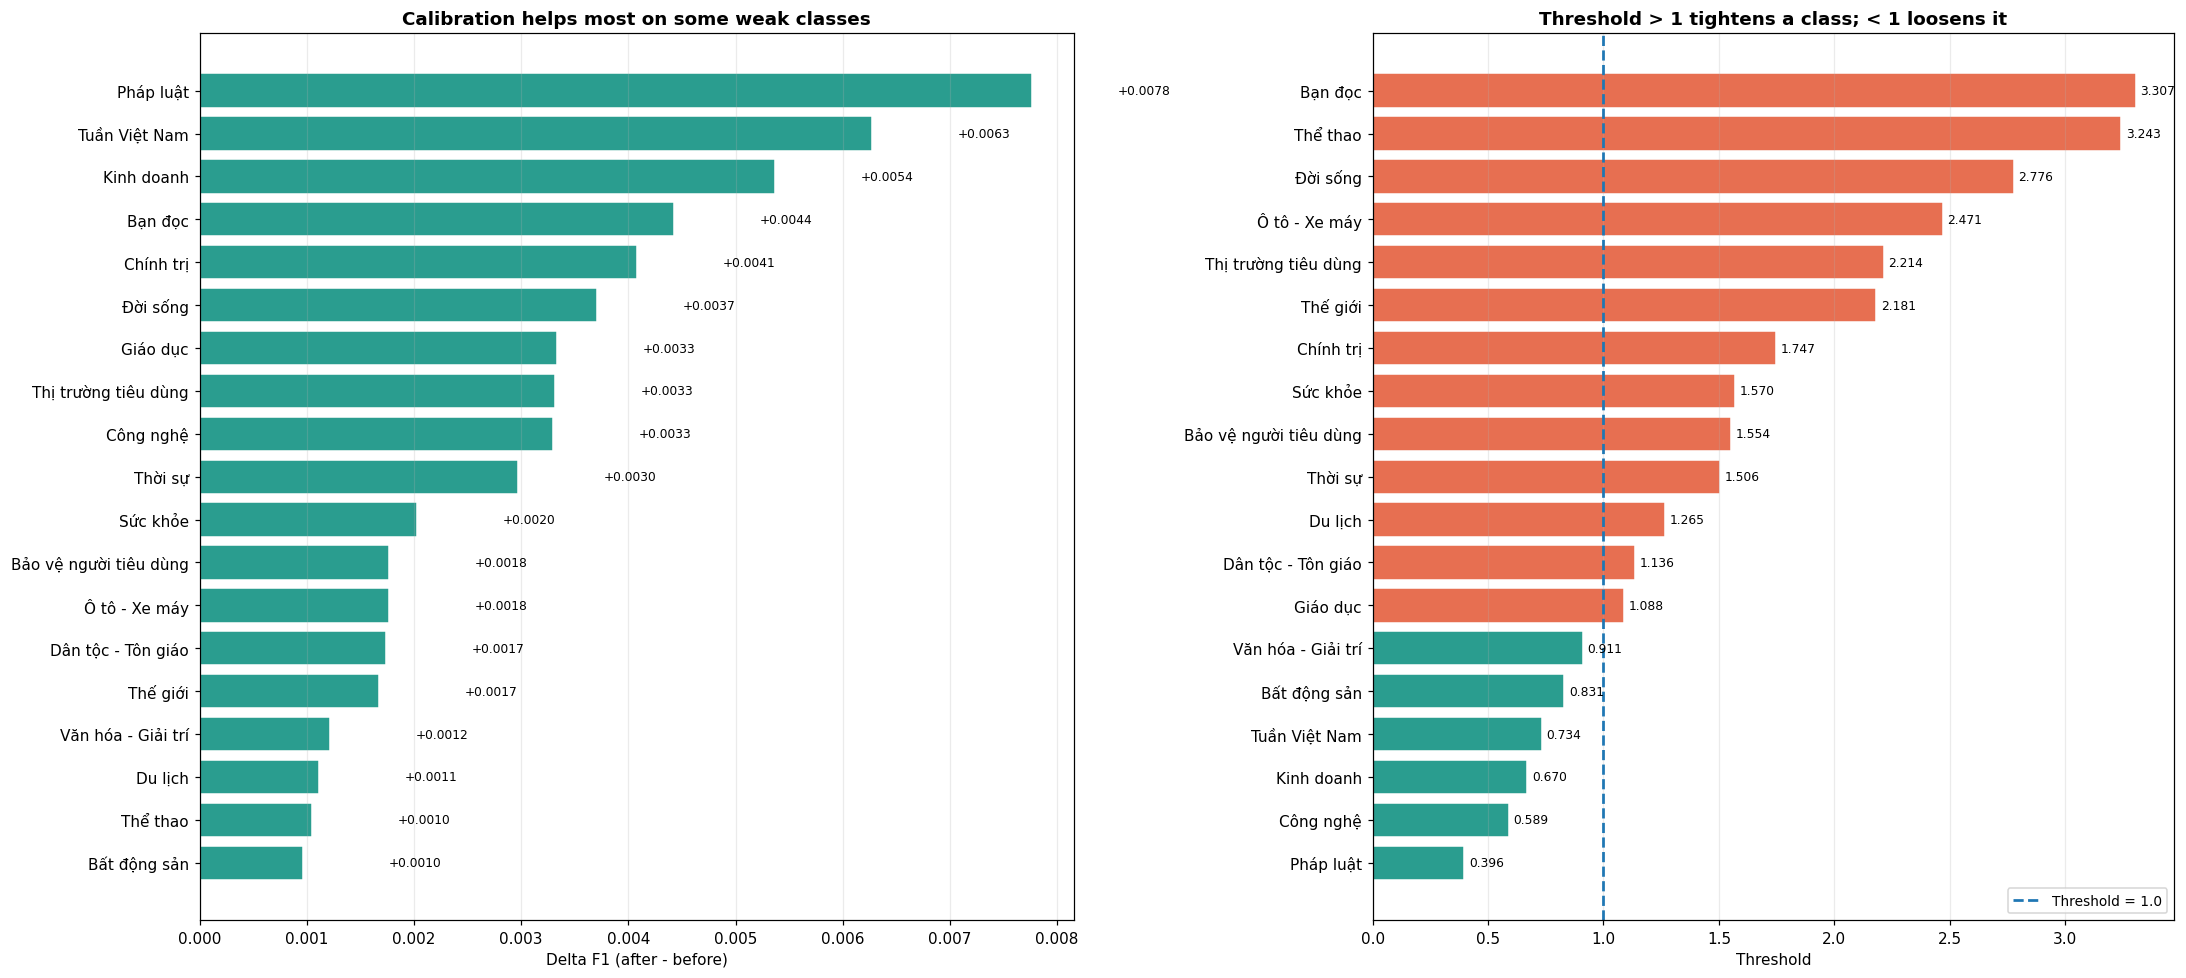
\includegraphics[width=\textwidth]{reused/figures/06_threshold_calibration.png}
\caption{Mức đổi F1 và ngưỡng theo lớp, nguyên hình từ notebook. Kết quả được tìm và đo trên cùng tập calibration.}\end{figure}

\section{Lưu cấu hình -- Section 8.3}
\code{thresholds.json} ghi temperature, ngưỡng từng lớp, khoảng tìm kiếm, 200 ứng viên, ba lượt và các chỉ số trước/sau. \code{label_config.json} trỏ tới tệp này và bật cờ sử dụng calibration. \code{metrics.json}, \code{classification_report.json} và \code{confusion_matrix.json} được xuất cùng package; report và confusion JSON mô tả dự đoán \emph{sau} hiệu chỉnh, còn hình confusion ở Section 6 mô tả \emph{trước} hiệu chỉnh.

Notebook cũ tìm $T$ và ngưỡng bằng chính nhãn của tập 31.906 bài đã dùng chọn checkpoint. Vì vậy, mức tăng sau calibration là kết quả hiệu chỉnh trên tập đã tham gia tối ưu. Một thiết kế tiếp theo cần giữ riêng train, validation để chọn checkpoint/calibration và test cuối cùng; không chuyển các điểm hiện tại thành kết quả của thiết kế ba tập chưa chạy.

\chapter{Chẩn đoán, giới hạn và tái lập}
\section{Phân tích lỗi -- Section 9}
Sau hiệu chỉnh, Dân tộc -- Tôn giáo vẫn là lớp thấp nhất với F1 0,7813, precision 0,7372 và recall 0,8310. Ngưỡng không giải quyết được toàn bộ khác biệt ngữ nghĩa hoặc độ bao phủ mẫu của lớp này. Các lớp có recall thấp gồm Thời sự, Thị trường tiêu dùng và Đời sống; việc tăng precision bằng ngưỡng cao đồng thời bỏ sót thêm bài thật của lớp.

\begin{table}[htbp]\centering\small
\begin{tabularx}{\textwidth}{XXrr}\toprule
Nhãn thực & Dự đoán & Số lỗi & Tỷ lệ trong lớp\\\midrule
Thời sự & Pháp luật & 236 & 12.58\%\\
Thị trường tiêu dùng & Kinh doanh & 127 & 9.10\%\\
Đời sống & Du lịch & 125 & 6.66\%\\
Kinh doanh & Bất động sản & 64 & 3.41\%\\
Bất động sản & Kinh doanh & 60 & 3.21\%\\
Chính trị & Dân tộc - Tôn giáo & 56 & 2.99\%\\
Thời sự & Chính trị & 55 & 2.93\%\\
Đời sống & Kinh doanh & 54 & 2.88\%\\
\bottomrule\end{tabularx}

\caption{Tám cặp nhầm lẫn lớn nhất sau hiệu chỉnh, tính từ confusion JSON. Tỷ lệ lấy trên số bài thật của lớp ở cột đầu.}\end{table}
Cặp Thời sự $\rightarrow$ Pháp luật có 236 lỗi, chiếm 12,58\% lớp Thời sự trong tập đánh giá. Thị trường tiêu dùng $\rightarrow$ Kinh doanh có 127 lỗi; Đời sống $\rightarrow$ Du lịch có 125 lỗi. Bước tiếp theo phù hợp là đọc các bài thuộc những cặp này, rà tiêu chí chuyên mục và đánh giá lại ảnh hưởng của class weight cùng ngưỡng trên validation riêng.

\section{Giới hạn của kết quả}
Thực nghiệm có một split với seed 42, không có độ lệch chuẩn qua nhiều seed. Corpus chưa được chia theo thời gian hoặc nhóm bài trùng. Bộ dữ liệu tải trong lần chạy không được pin revision, và cache không chứa đầy đủ chữ ký nội dung nguồn. Audit của bộ 7.600 tiêu đề không thay thế được việc kiểm tra split của lần fine-tune cũ.

Log khi Trainer nạp lại checkpoint ghi cảnh báo tên khóa LayerNorm dạng beta/gamma và weight/bias. Cảnh báo này làm hạn chế khả năng khẳng định quá trình nạp lại đã khôi phục mọi tensor đúng như mong đợi. Notebook và số đo được giữ nguyên; một lần tái lập mới cần kiểm tra danh sách missing/unexpected keys, thống nhất phiên bản Transformers và xử lý tương thích checkpoint trước khi đo lại.

Chỉ số sau hiệu chỉnh được kiểm tra lại từ confusion đã lưu, không suy ra rằng đã chạy lại toàn bộ model trên dữ liệu nguồn. Raw logits, prediction từng bài và ID split của lần chạy cũ chưa có trong package, nên chưa tái kiểm được NLL/ECE từ logits hoặc membership từng bản ghi. Các số NLL/ECE, đường cong và thống kê độ dài được truy về output notebook.

\section{Tệp và lệnh kiểm tra}
\code{notebooks/text.ipynb} giữ nguyên file train full đã chạy, gồm code, output và bảy hình. Đọc output không thực hiện huấn luyện; chọn Run All trong runtime mới có thể tải dữ liệu và fine-tune đầy đủ theo cấu hình Section 0.3. Các đường dẫn trong notebook dành cho workspace chạy thí nghiệm, nên cần chọn thư mục riêng trước khi chạy lại.

\code{python -m text_reuse.analysis} kiểm tra SHA256 17 tệp nhập, gồm notebook, hình và metadata, rồi tính lại accuracy, macro-F1, weighted-F1 và chỉ số từng lớp từ confusion sau hiệu chỉnh. \code{python -m text_reuse.analysis --export} xuất lại các bảng và hình epoch cho báo cáo. Lệnh biên dịch là \code{python scripts/build_report.py --track text}. Nguồn nhập và checkpoint identity được ghi trong \code{reports/text/reuse-manifest.json}.

Báo cáo sử dụng AI được đính kèm tại tệp \code{AI_USE_REPORT.md} trong repository.

\appendix
\chapter{Bộ đối chứng trên tiêu đề}
Thực nghiệm bổ sung dùng 7.600 tiêu đề cân bằng, lấy sau audit corpus hiện tại, chia train/validation/test 5.320/1.140/1.140. PhoBERT đóng băng tạo vector 768 chiều rồi Logistic Regression được fit trên train. Các baseline TF-IDF và classifier được chọn cấu hình theo validation, sau đó đo trên test riêng.
\begin{table}[H]\centering\small
\begin{tabularx}{\textwidth}{Xrr}\toprule
Mô hình & Accuracy & Macro-F1\\\midrule
Majority & 5,26\% & 0,0053\\
TF-IDF từ + Linear SVM & 66,32\% & 0,6582\\
TF-IDF ký tự + Linear SVM & 67,28\% & 0,6676\\
PhoBERT đóng băng + Logistic Regression & 77,54\% & 0,7738\\\bottomrule
\end{tabularx}
\caption{Các phép đo bổ sung trên 1.140 tiêu đề test.}\end{table}
Không dùng chênh lệch giữa 77,54\% và 90,52\% để kết luận lợi ích riêng của fine-tuning: hai thí nghiệm khác input, số mẫu, phân bố lớp và vai trò tập đánh giá. Notebook đối chứng ở \code{notebooks/text_baselines.ipynb}; báo cáo chi tiết ở \code{reports/text/baselines.pdf}. Các bằng chứng mới này tiếp tục được kiểm tra bằng \code{python -m studies.audit --models}.

\chapter{Hình gốc và đối chiếu nguồn}
Bảy hình được trích trực tiếp từ output notebook, không vẽ lại từ các bộ kết quả khác. Các hình được đặt ở các phần tương ứng hoặc dưới đây; hình đường cong gốc được giữ để đối chiếu, còn phần phân tích dùng hình vẽ lại theo epoch vì hình gốc đặt mốc eval epoch trên trục train step.
\begin{figure}[htbp]\centering
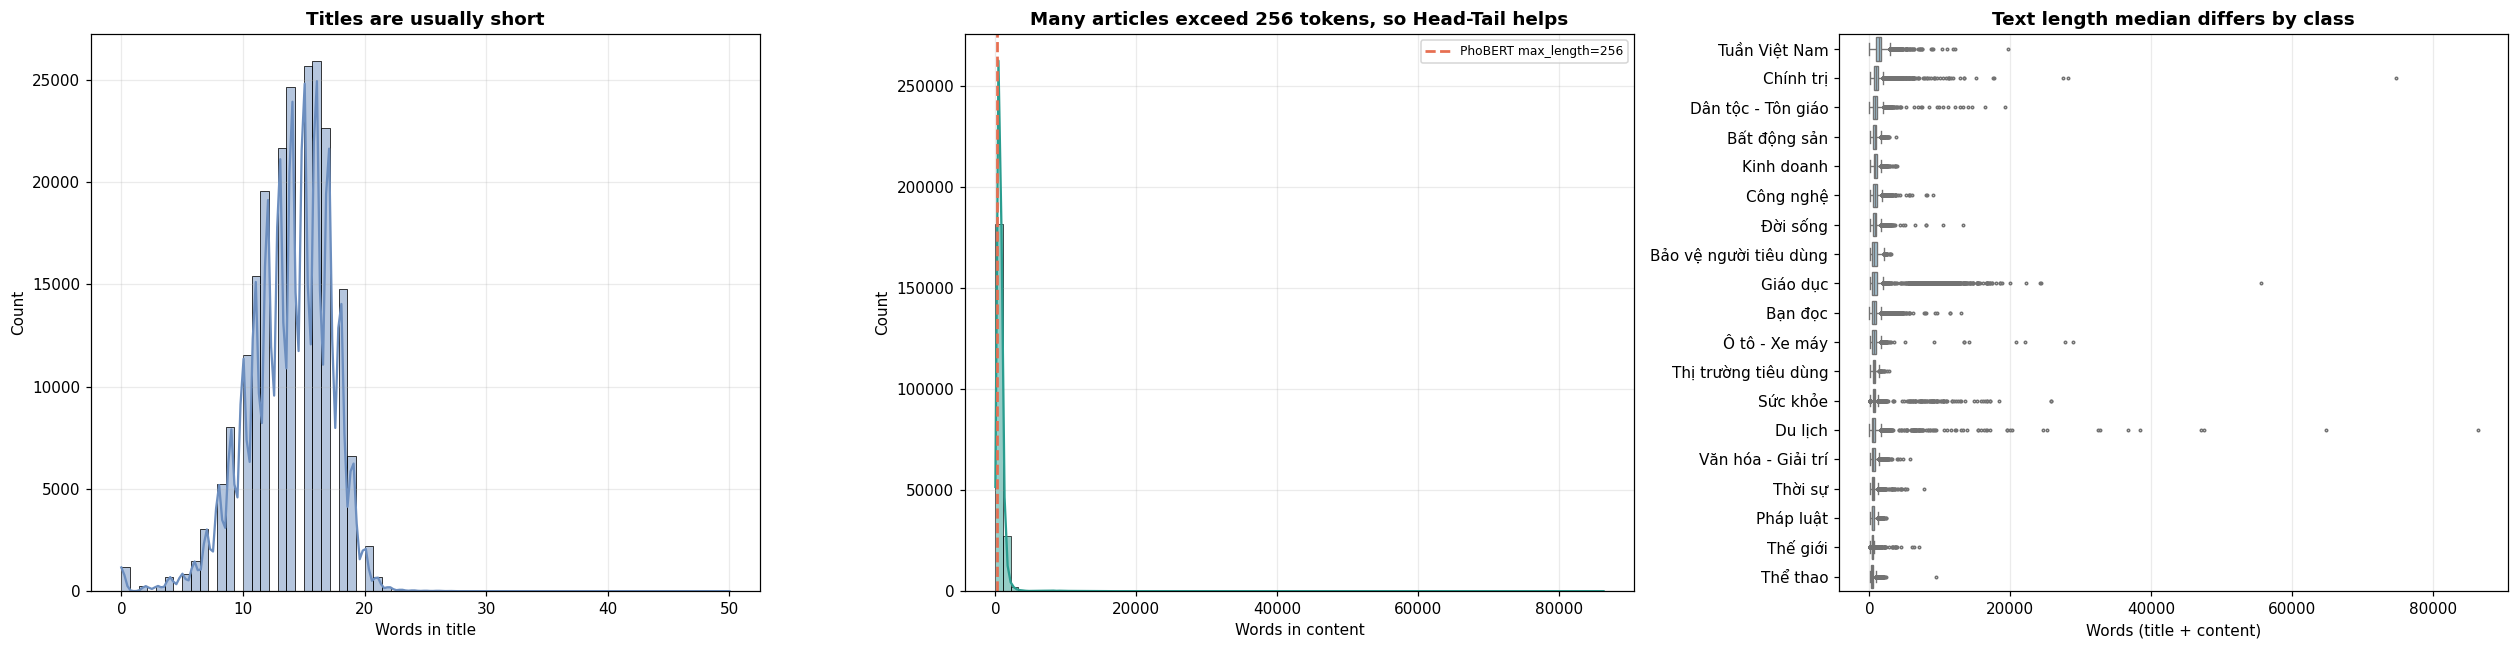
\includegraphics[width=.9\textwidth]{reused/figures/02_text_length.png}
\caption{Histogram độ dài tiêu đề, nội dung và phân bố theo chuyên mục. Đường 256 trên trục số từ chỉ là mốc tham chiếu; giới hạn thực của mô hình được kiểm tra lại bằng tokenizer.}\end{figure}
\begin{figure}[htbp]\centering
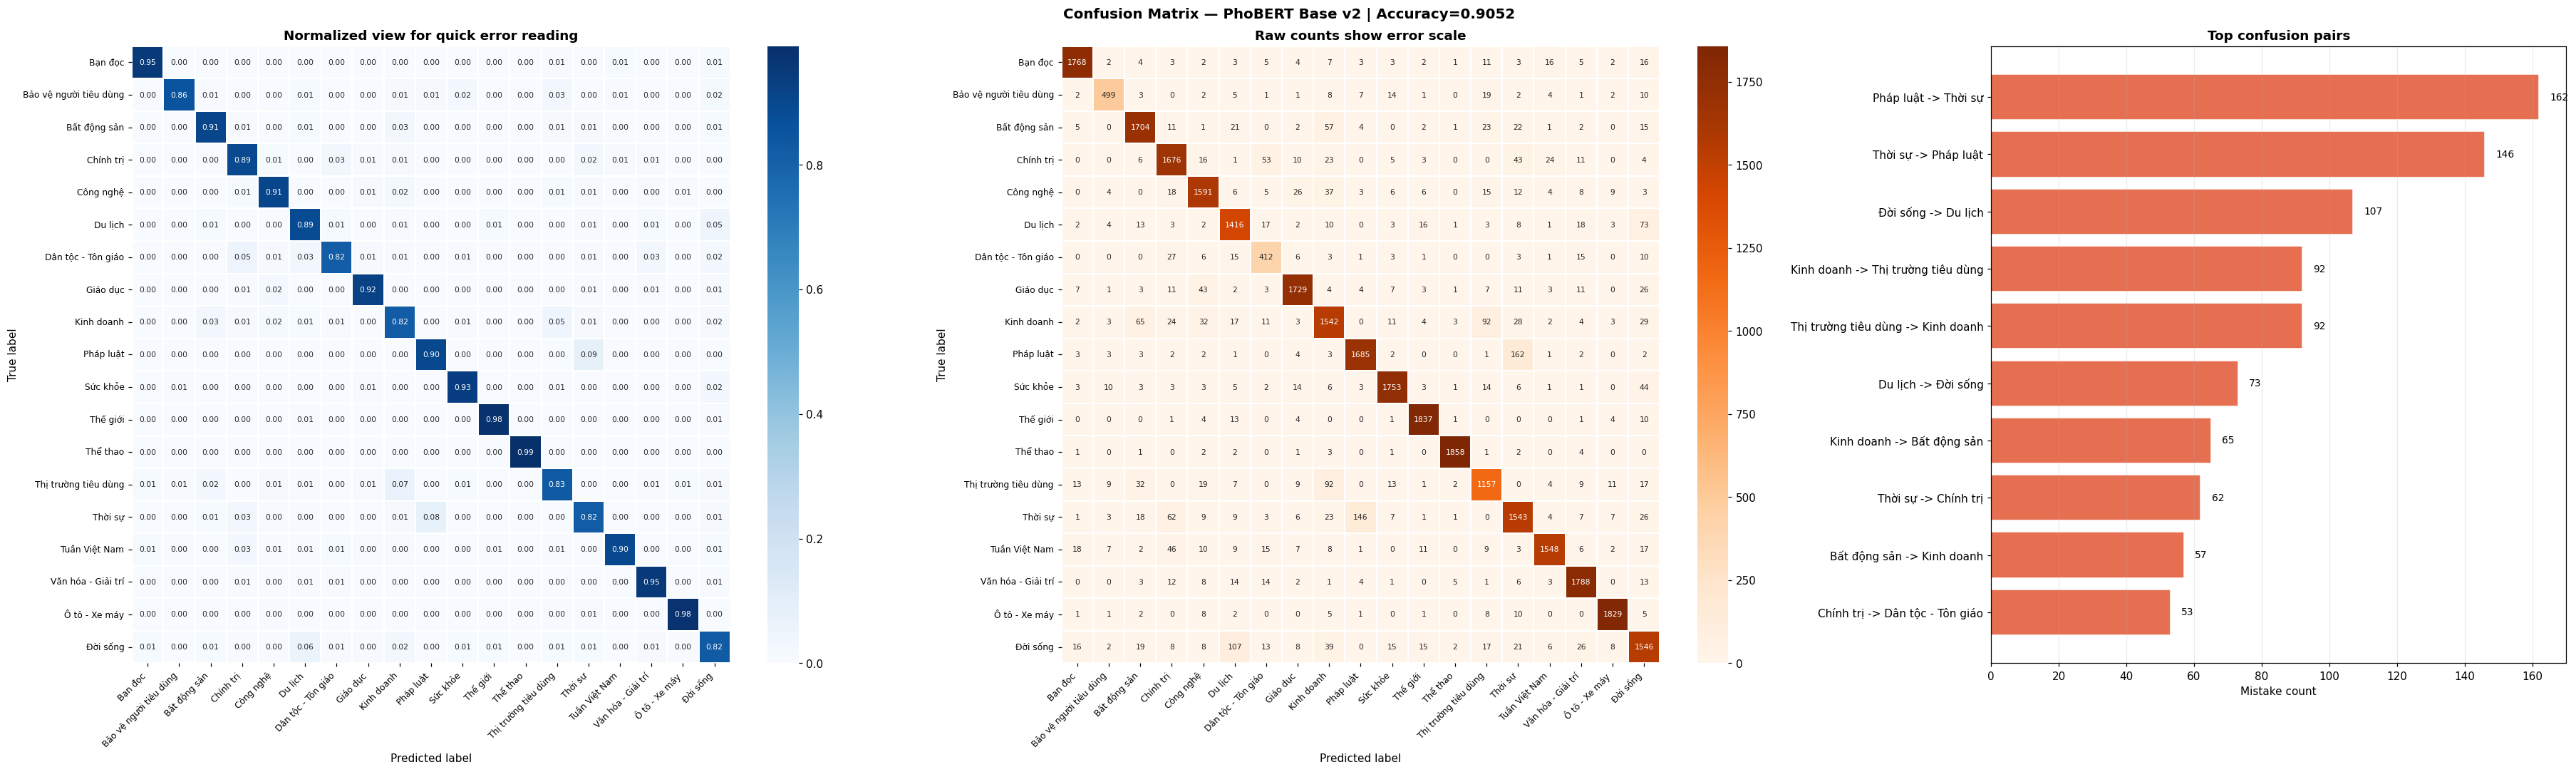
\includegraphics[width=.9\textwidth]{reused/figures/03_confusion_matrix.png}
\caption{Confusion trước calibration: chuẩn hóa theo hàng, số lỗi và cặp nhầm lẫn. Bản gốc độ phân giải đầy đủ nằm trong thư mục figures.}\end{figure}
\begin{figure}[htbp]\centering
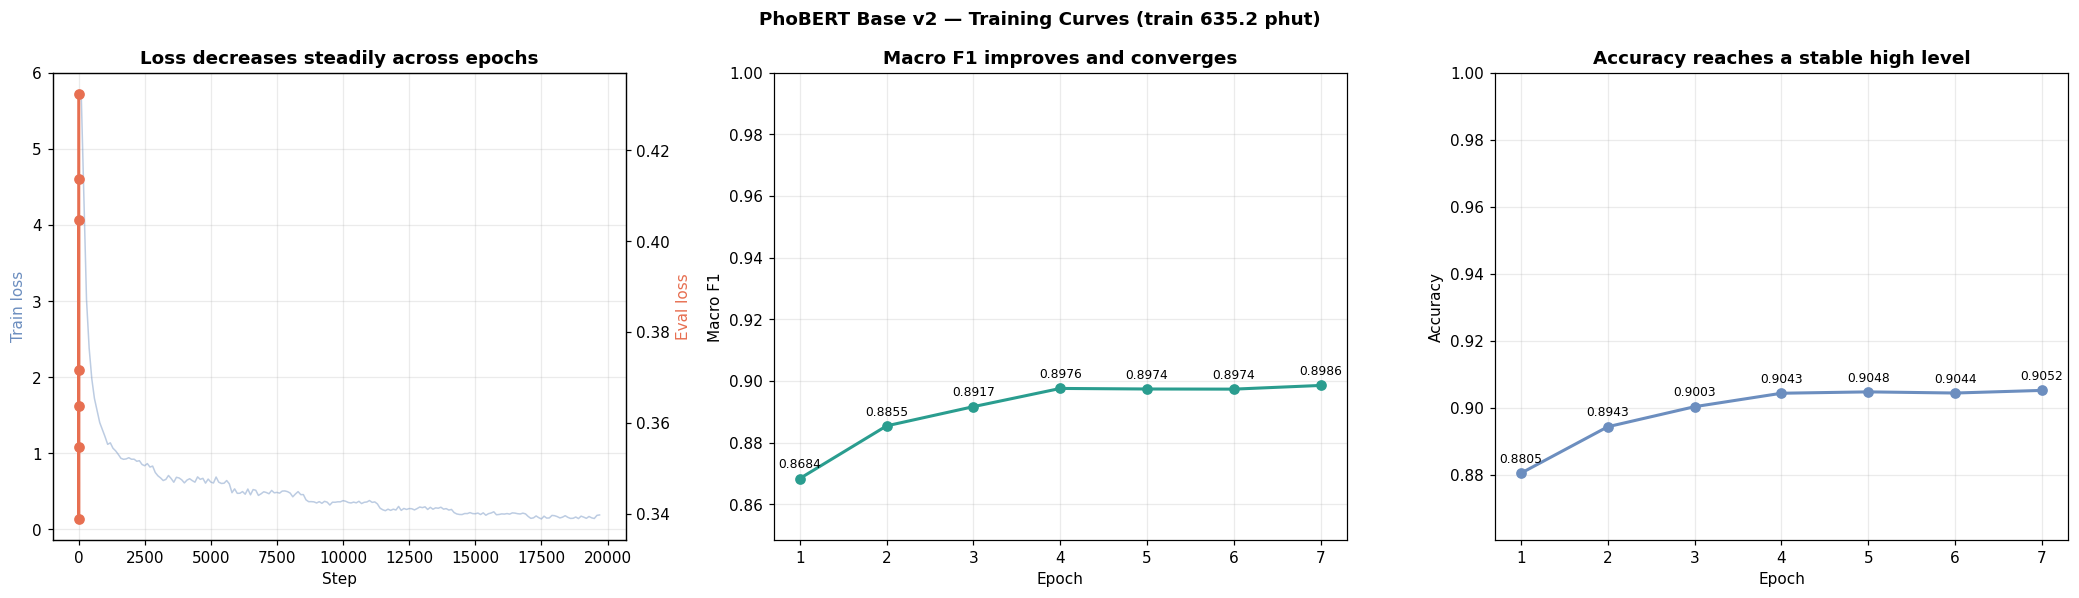
\includegraphics[width=.9\textwidth]{reused/figures/05_training_curves.png}
\caption{Hình đường cong gốc của notebook. Ở ô loss, đường eval dùng epoch còn đường train dùng step; không đọc vị trí hai đường theo cùng đơn vị trục ngang.}\end{figure}

\begin{thebibliography}{9}\addcontentsline{toc}{chapter}{Tài liệu tham khảo}
\bibitem{vietnamnet} Huỳnh Thành Đạt. \emph{VietnamNet News}. \url{https://huggingface.co/datasets/dathuynh1108/vietnamnet-news}.
\bibitem{application} Huỳnh Thành Đạt. \emph{PhoBERT News Classification App}. Notebook và model package tại commit e171688. \url{https://github.com/dathuynh1108/phobert-news-classification-app}.
\bibitem{phobert} D. Q. Nguyen và A. T. Nguyen. \emph{PhoBERT: Pre-trained language models for Vietnamese}. Findings of EMNLP, 2020. \url{https://huggingface.co/vinai/phobert-base-v2}.
\bibitem{pyvi} PyVi. Vietnamese word segmentation. \url{https://pypi.org/project/pyvi/}.
\bibitem{transformers} Hugging Face. Transformers: Trainer, TrainingArguments và sequence classification. \url{https://huggingface.co/docs/transformers/}.
\bibitem{pytorch} PyTorch. CrossEntropyLoss. \url{https://pytorch.org/docs/stable/generated/torch.nn.CrossEntropyLoss.html}.
\end{thebibliography}

\end{document}
